\section{Introduction}

Recently, Linux containers have drawn significant amount of attention because they are lightweight, portable, and repeatable.
Linux containers are generally more lightweight than virtual machine (VM) clusters, 
because the containers share the kernel with the host operating system (OS), even though they maintain separate execution environments. 
They are generally portable because the process execution environments are archived into tar files, 
so whenever one attempts to run a container, the exact same file systems are restored from the archives 
even when totally different data centers are used. 
This means that containers can provide repeatable and portable execution environments.
%
For the same reasons, Linux containers are attractive for web services as well, 
and it is expected that web services consisting of container clusters would be 
capable of being migrated easily for variety of purposes. For example disaster recovery, 
cost performance improvemets, legal compliance, and shortening the geographical distance to customers 
are the main concerns for web service providers in e-commece, gaming, Financial technology(Fintech) and Internet of Things(IoT) field.
%

Kubernetes\cite{K8s2017}, which is one of the popular container cluster management systems, 
enables easy deployment of container clusters.
Since Kubernetes hides the differences in the base environments, users can easily deploy a web service on different 
cloud providers or on on-premise data centers, without adjusting the container cluster configurations to the new environment. 
This allows a user to easily migrate a web service consisting of a container cluster even to the other side of the world. 
A user starts the container cluster in the new location, route the traffic there, 
then stop the old container cluster at his or her convenience.
This is a typical web service migration scenario.

However, this scenario only works when the user migrates a container cluster among major cloud providers including Google Cloud Platform (GCP), 
Amazon Web Services (AWS), and Microsoft Azure.
The Kubernetes does not include a load balancer, and is heavily dependent on external load balancers that are set up on the fly 
by cloud providers through their application protocol interfaces (APIs). 
These external load balancers distribute incoming traffic to every server that hosts containers.
The traffic is then distributed again to destination containers using iptables destination 
network address translation (DNAT)\cite{MartinA.Brown2017,Marmol2015} rules in a round-robin manner. 
The problem happens in the environment with a load balancer that is not supported by the Kubernetes, 
e.g. in an on-premise data center with a bare metal load balancer. 
In such environments, the user needs to manually configure 
the static route for inbound traffic in an ad-hoc manner. 
Since the Kubernetes fails to provide an uniform environment from a container cluster view point,
migrating container clusters among the different environments will always be a burden.

In order to solve this problem by eliminating the dependency on external load balancer,
herein we propose a containerized software load balancer that is run by Kubernetes as  
as a part of web services consisting of container cluster.
It enables a user to easily deploy a web service on different environment without modification, 
because the load balancer is included in the web service itself. 
To accomplish this, we will containerize Linux kernel's Internet Protocol Virtual Server (IPVS)\cite{Zhang2000} 
Layer 4 load balancer using an existing Kubernetes ingress\cite{K8sIngress2017} framework, as a proof of concept.
%
%
To prove that our approach will not significantly deteriorate the performance,  
we will also compare the performance of our proposed load balancer with those of 
iptables DNAT load balancer and the Nginx Layer 7 load balancing. 
%
The results indicated that the proposed load balancer could improve the portability of container clusters 
without performance degradation compared with the existing load balancer.
The performance of the proposed load balancer may be affected by the network configurations of overlay network 
and distributed packet processing. 
We also evaluate how the network configurations affects the performance and discusses 
the best setting that derives the best performance.

The contributions of this paper are as follows: 
1) We propose a portable software load balancer that is runnable on any cloud provider, or on on-premise data centers, 
as a part of a container cluster.
2) We discuss feasibility of the proposed load balancer by comparing its performance with other load balancers.
3) We also discuss usable overlay network configurations and clarify the importance of techniques 
that will  draw the best performance from such load balancers.  

The rest of the paper is organized as follows.
Section \ref{Related Work} highlights work that deals specifically with container cluster migration, 
software load balancer containerization, and load balancer related tools within the context of the container technology. 
Section \ref{Load balancers in Kubernetes cluster} will explain existing architecture problems and propose our solutions.
In Section \ref{Performance Measurement}, experimental conditions and the parameters 
that we considered to be important in our experiment will be described in detail.
Then, we will show our experimental results and discuss the obtained performance characteristics in Section~\ref{Result and Discussion},  
which is followed by a summary of our work in Section~\ref{Conclusions}.

\section{Related Work}\label{Related Work}

This section highlights related work, especially that dealing with container cluster migration, 
software load balancer containerization, load balancer tools within the context of the container technology and scalable load balancer in the cloud providers.

\paragraph{\bf Container cluster migration:}

Kubernetes developers are trying to add federation\cite{K8sFederation2017} capability for handling situations 
where multiple Kubernetes clusters\footnote{The {\em Kubernetes cluster} refers to a server cluster 
controlled by the Kubernetes container management system, in this paper.} 
are deployed on multiple cloud providers or on-premise data centers, 
and are managed via the Kubernetes federation API server (federation-apiserver). 
However, how each Kubernetes cluster is run on different types of cloud providers
and/or on-premise data centers, especially when the load balancers of such environments are not supported by Kubernetes, 
seems beyond the scope of that project. 
The main scope of this paper is to make Kubernetes usable in environments 
without supported load balancers by providing a containerized software load balancer.

\paragraph{\bf Software load balancer containerization:}
As far as load balancer containerization is concerned, the following related work has been identified:
Nginx-ingress\cite{Pleshakov2016,NginxInc2016} utilizes the ingress\cite{K8sIngress2017} capability of Kubernetes, 
to implement containerized Nginx proxy as a load balancer. Nginx itself is famous as a high-performance web server program
that also has the functionality of a Layer-7 load balancer. Nginx is capable of handling Transport Layer Security(TLS) encryption, 
as well as Uniform Resource Identifier(URI) based switching. However, the flip side of Nginx is that it is much slower than Layer-4 switching.
We compared the performance between Nginx as a load balancer and our proposed load balancer in this paper.
%
Meanwhile, the kube-keepalived-vip\cite{Prashanth2016} project is trying to use Linux kernel's IPVS\cite{Zhang2000} 
load balancer capabilities by containerizing the keepalived\cite{ACassen2016}.
The kernel IPVS function is set up in the host OS's net name spaces and is shared among multiple web services,
as if it is part of the Kubernetes cluster infrastructure.
Our approach differs in that the IPVS rules are set up in container's net name spaces 
and function as a part of the web service container cluster itself.
The load balancers are configurable one by one, and are  movable with the cluster once the migration is needed.
The kube-keepalived-vip's approach lacks flexibility and portability whereas ours provide them.
%
The swarm mode of the Docker\cite{DockerCoreEngineering2016,DockerInc2017} also uses IPVS for internal load balancing,
but it is also considered as part of Docker swarm infrastructure, 
and thus lacks the portability that our proposal aims to provide.

\paragraph{\bf Load balancer tools in the container context:}
There are several other projects where efforts have been made to utilize IPVS in the context of container environment.
For example, GORB\cite{Sibiryov2015} and clusterf\cite{Aaltodoc:http://urn.fi/URN:NBN:fi:aalto-201611025433} are daemons 
that setup IPVS rules in the kernel inside the Docker container. 
They utilize running container information stored in key-value storages
like Core OS etcd\cite{CoreOSEtcd} and HashiCorp's Consul\cite{HashiCorpConsul}. 
Although these were usable to implement a containerized load balancer in our proposal, we did not use them, 
since Kubernetes ingress framework already provided the methods to retrieve running container information through standard API.

\paragraph{\bf Cloud load balancers:}

As far as the cloud load balancers are concerned, two articles have been identified.
Google's maglev\cite{eisenbud2016maglev} is a software load balancer used in Google Cloud Platform(GCP)\cite{Voellm2013}.
Maglev uses modern technologies including per flow ECMP and kernel bypass for userspace packet processing.
Maglev serves as the GCP's load balancer that is used by the Kubernetes.
Maglev can be solely used in GCP, and the users need open source software load balancer that is runnable even in on-premise data centers.
Microsoft's Ananta\cite{patel2013ananta} is another software load balancer implementation using ECMP and windows network stack.
Ananta can be solely used in Microsoft's Azure cloud infrastructure\cite{patel2013ananta}.
The proposed load balancer by the author is different in that it is aimed to be used in every cloud provider and on-premise data centers.

\section{Proposed Architecture}\label{Architecture}



\section{Implementation}\label{Implementation}

\section{Evaluation}\label{Evaluation}

\subsection{Functionality}\label{Functionality}

\subsection{Performance}\label{Performance}


\subsection{Overview}\label{Network}
Here we discuss overall architecture of the proposed load balancer.
\begin{figure}
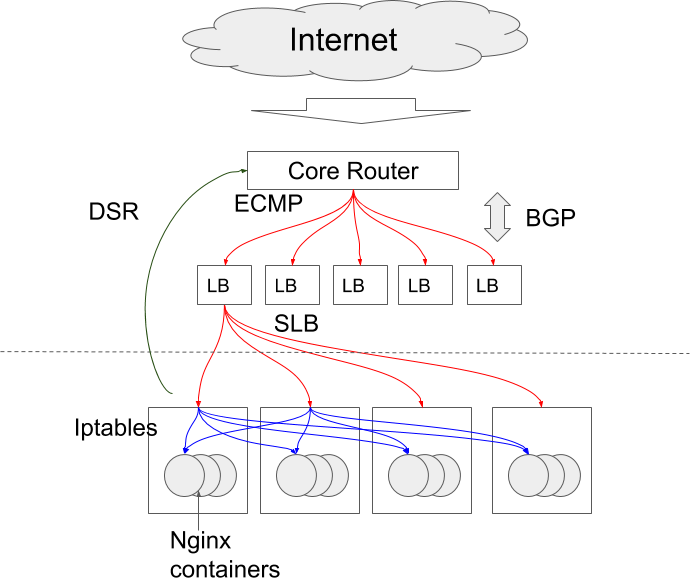
\includegraphics[width=\columnwidth]{Figs/google_lb.png}
\caption{Conventional architecture. Software load balancers are set up via cloud API. }
\label{fig:google_lb}
\end{figure}
Figure~\ref{fig:google_lb} show conventional architecture of the container cluster infrastructure, e.g. Kubernetes.
Below the dotted line, there are node Linux machines that hosts containers, which is controlled by Kubernetes.
Above the dotted line, there are Software Load Balancers(SLBs) and the core router.
All the equipment and software entities above the dotted line are controlled by base cloud infrastructure.

Upon launch of the container clusters, SLBs are set up by the cloud infrastructure.
At the same time iptables DNAT rule's are set up on each of the node Linux machines.
These SLBs distribute incoming traffic to every node that hosts containers.
The traffic is then distributed again to destination containers using iptables destination 
network address translation (DNAT)\cite{MartinA.Brown2017,Marmol2015} rules in a round-robin manner. 

\begin{figure}
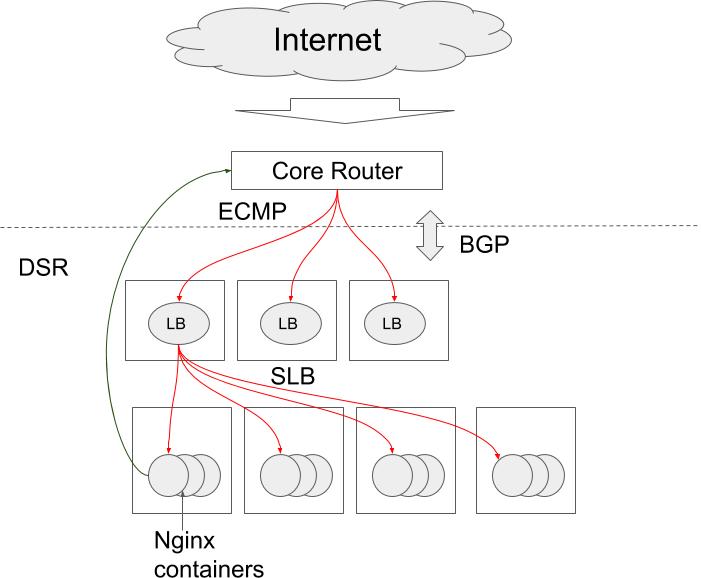
\includegraphics[width=\columnwidth]{Figs/new_lb}
\caption{Proposed architecture. Routing table of the Core Router is updated via BGP.}
\label{fig:new_lb}
\end{figure}

Figure~\ref{fig:new_lb} shows proposed architecture.
Upon launch of the container clusters, SLBs are also launched as a part of the container cluster.
Then, the SLBs communicate with the Core router using the Border Gateway Protocol(BGP)\cite{rekhter2005border} to update routing table.
The core router evenly distributes the incoming traffic to SLBs, then the SLB directly forward the traffic to destination containers.

The big differences between the conventional architecture and the proposed ones are;
a) iptables DNAT load balancing layer does not exist in the latter,
b) while the communication between the Kubernetes and the cloud provider in the conventional architecture is the vendor specific API requests to setup the external SLBs, the communication between the Kubernetes and the cloud provider is standard BGP protocol in the proposed architecture.

In other words, the proposed architecture is better than the conventional one, because it eliminates one extra network hop and communicate with external world using standard protocol.
And also because the SLBs are containerized and are the part of the cluster, a service can be deployed in any environment including on-premise data centers, if only the core router permits the update of its routing table via BGP.
This will greatly improve the portability compared to the conventional architecture where the support for vendor specific API is always required.

\subsection{Containerization}\label{IPVS}

Here we discuss containerization of a software load balancer.
We designed the proposed load balancer using three components, IPVS, keepalived, and a controller. 
These components are placed in a Docker container image.
The IPVS is a Layer-4 load balancer capability, which is included in the Linux kernel 2.6.0 released in 2003 or later, 
to distribute incoming Transmission Control Protocol(TCP) traffic to 
{\em real servers}\footnote{The term, {\em real servers} refers to worker servers that will respond to incoming traffic, 
in the original literature\cite{Zhang2000}. We will also use this term in the similar way.}\cite{Zhang2000}. 
For example, IPVS distributes incoming Hypertext Transfer Protocol(HTTP) traffic destined for a single destination IP address, 
to multiple HTTP servers(e.g. Apache HTTP or Nginx) running on multiple nodes in order to improve the performance of web services.
Keepalived is a management program that performs health checking for {\em real servers}
and manage IPVS balancing rules in the kernel accordingly.
It is often used together with IPVS to facilitate ease of use.
Although keepalived also supports Virtual Router Redundancy Protocol(VRRP)\cite{hinden2004virtual}, the authors plans to use ECMP to achieve the redundancy.
The controller is a daemon that periodically monitors the {\em pod} information on the master, 
and performs various actions when such information changes.
Kubernetes provides ingress controller framework as the Go Language(Golang) package to implement such controllers. 
We have implemented a controller program that will feed {\em pod} state changes to keepalived 
using this framework. 

\begin{figure}
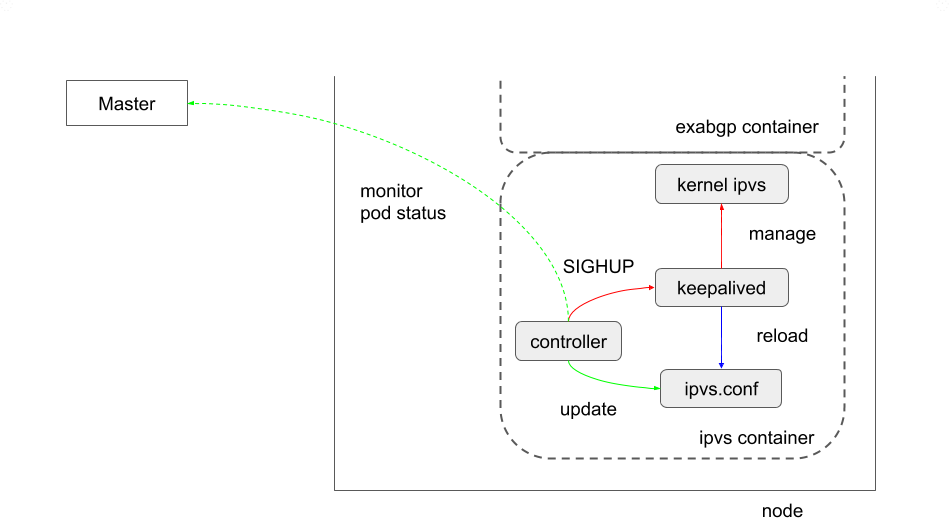
\includegraphics[width=\columnwidth]{Figs/ipvs-ingress-schem}
\caption{Implementation}
\label{fig:IPVS-ingress-schem}
\end{figure}

The proposed load balancer needs to dynamically reconfigure the IPVS balancing rules whenever {\em pods} are created/deleted. 
Figure~\ref{fig:IPVS-ingress-schem} is a schematic diagram to show the dynamic reconfiguration of the IPVS rules.
The right part of the figure shows the enlarged view of one of the nodes where the load balancer pod(LB2) is deployed.
Two daemon programs, controller and keepalived, run in the container inside the LB2 pod are illustrated.
The keepalived manages Linux kernel's IPVS rules depending on the ipvs.conf configuration file.
It is also capable of health-checking the liveliness of {\em real server}, 
which is represented as a combination of the IP addresses and port numbers of the target {\em pods}. 
If the health check to a {\em real server} fails, keepalived will remove that {\em real server} from the IPVS rules.

The controller monitors information concerning the running {\em pods} of a service 
in the Kubernetes cluster by consulting the apiserver running on the master.
Whenever {\em pods} are created or deleted, the controller will automatically regenerate an appropriate ipvs.conf 
and issue SIGHUP to keepalived.
Then, keepalived will reload the ipvs.conf and modify the kernel's IPVS rules accordingly.
The actual controller\cite{ktaka_ccmp_2017_826894} is implemented using the Kubernetes ingress controller\cite{K8sIngress2017} framework. 
By importing existing Golang package, \enquote{k8s.io/ingress /core/pkg/ingress}, we could simplify the implementation, e.g. 
120 lines of code.  

\subsection{XDP load balancer}\label{XDP loadbalancer}
Even though we could successfully containerize the load balancers and could deploy it as a part of web service,
the performance we obtained was not equivalent that of scalable load balancers provided by the GCP.
We will discuss ongoing work as to how to improve the performance levels of the open source software load balancer using the novel XDP technology.

The IPVS is implemented as kernel modules that attach the Netfilter's\cite{hubert2002linux} hooks and heavily dependent on Linux kernel's standard network stack.
The IP packet processing of the Linux kernel has been claimed to be inefficient, and thus unable to meet the speed requirement of 10Gbps and above.
Several alternative techniques, DPDK\cite{dpdkorg}, netmaps\cite{rizzo2012netmap}, PF\_RING\cite{deri2004improving} and Maglev\cite{eisenbud2016maglev} to increase the speed of the packet processing have been proposed.

Most bypass the Linux kernel network stack and process the packet in user spaces.
While they may improve the performance level in specific applications, they all have some issues regarding compatibility because of the bypass.
Often they require dedicated physical NIC, other than the ones used for standard Linux services, e.g., ssh.

Recently, the Linux kernel introduced eXpress Data Plane (XDP)\cite{bertin2017xdp} a novel way to improve the traffic manipulation speed, while keeping compatibility with the other functions of the Linux standard networking stack.

By using the XDP infrastructure, a user can write code that manipulates traffic in the very early stage of accepting the packets from outside the Linux box.
It will enable a user to inject a bytecode into the kernel, let the kernel compile it into native machine code and then the code will manipulate the traffic only if it matches the predefined conditions.
Traffic that did not match the conditions are pass to the Linux kernel's standard networking stack.

We are now developing a software load balancer using XDP technology.
The design of such load balancer is also presented at the time of the presentation.

\section{Experiments}\label{Experiments}

We will now discuss the feasibility of the proposed load balancer by comparing 
its performance with those of existing iptables DNAT and the Nginx based load balancers. 
We conducted the performance measurements using the benchmark program called wrk\cite{Glozer2016}.
The following subsections explain these in further detail. 

\subsection{Benchmark method}

\begin{figure}
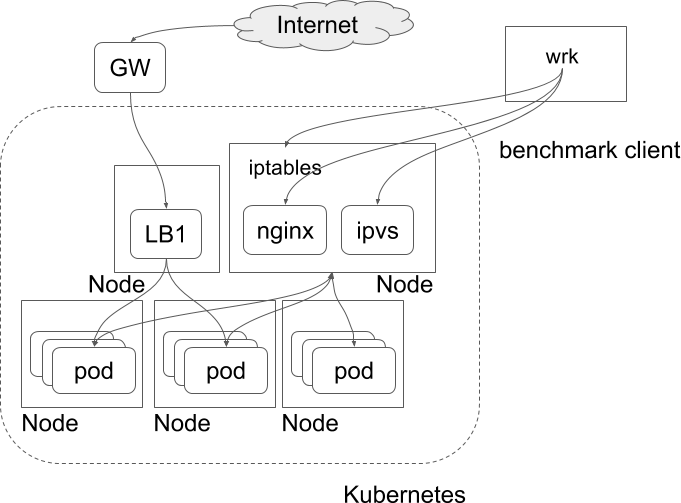
\includegraphics[width=\columnwidth]{Figs/benchmark-schem}
\caption{Benchmark setup}
\label{fig:benchmark-schem}
\end{figure}

We measured the performance of the load balancers using the wrk.
Figure~\ref{fig:benchmark-schem} illustrates a schematic diagram of our experimental setup.
Multiple {\em pods} are deployed on multiple nodes in the Kubernetes cluster. 
In each {\em pod}, a Nginx web server that returns the IP address of the {\em pod} are running.
We then set up the IPVS, iptables DNAT, and Nginx load balancers on one of the nodes(the top right node in the Figure~\ref{fig:benchmark-schem}). 

We measured the throughput, Request/sec, of the web service running on the Kubernetes cluster as follows:
The HTTP GET requests are sent out by the wrk on the client machine toward the nodes,
using destination IP addresses and port numbers that are chosen based on the type of the load balancer on which the measurement is performed.
The load balancer on the node then distributes the requests to the {\em pods}.
Each {\em pod} will return HTTP responses to the load balancer, after which the load balancer returns them to the client.
Based on the number of responses received by wrk on the client, 
load balancer performance, in terms of Request/sec can be obtained. 

\subsection{Benchmark results}

Figure~\ref{fig:IPVS-iptables-nginx_2figs} compares the performance measurement results 
among the IPVS, iptables DNAT, and Nginx load balancers
with the condition of \enquote{(RSS, RPS) = (off on)}.
The proposed IPVS load balancer exhibits almost equivalent performance as the existing iptables DNAT based load balancer. 
The Nginx based load balancer shows no performance improvement even though the number of the Nginx web server {\em pods} is increased.
It is understandable because the performance of the Nginx as a load balancer is expected to be similar to the performance as a web server.
Figure~\ref{fig:latency_cdf_rps_40pods} compares Cumulative Distribution Function(CDF) of the load balancer latency at the constant load.
The latencies are a little bit smaller for IPVS, however we consider the difference almost negligible.
For example, the median value at 160K[req/s] load for IPVS and iptables DNAT are, 1.1 msec and 1.2 msec, respectively.
So, we can conclude our proposed load balancer showed no performance degradation while providing potability.

\begin{figure}
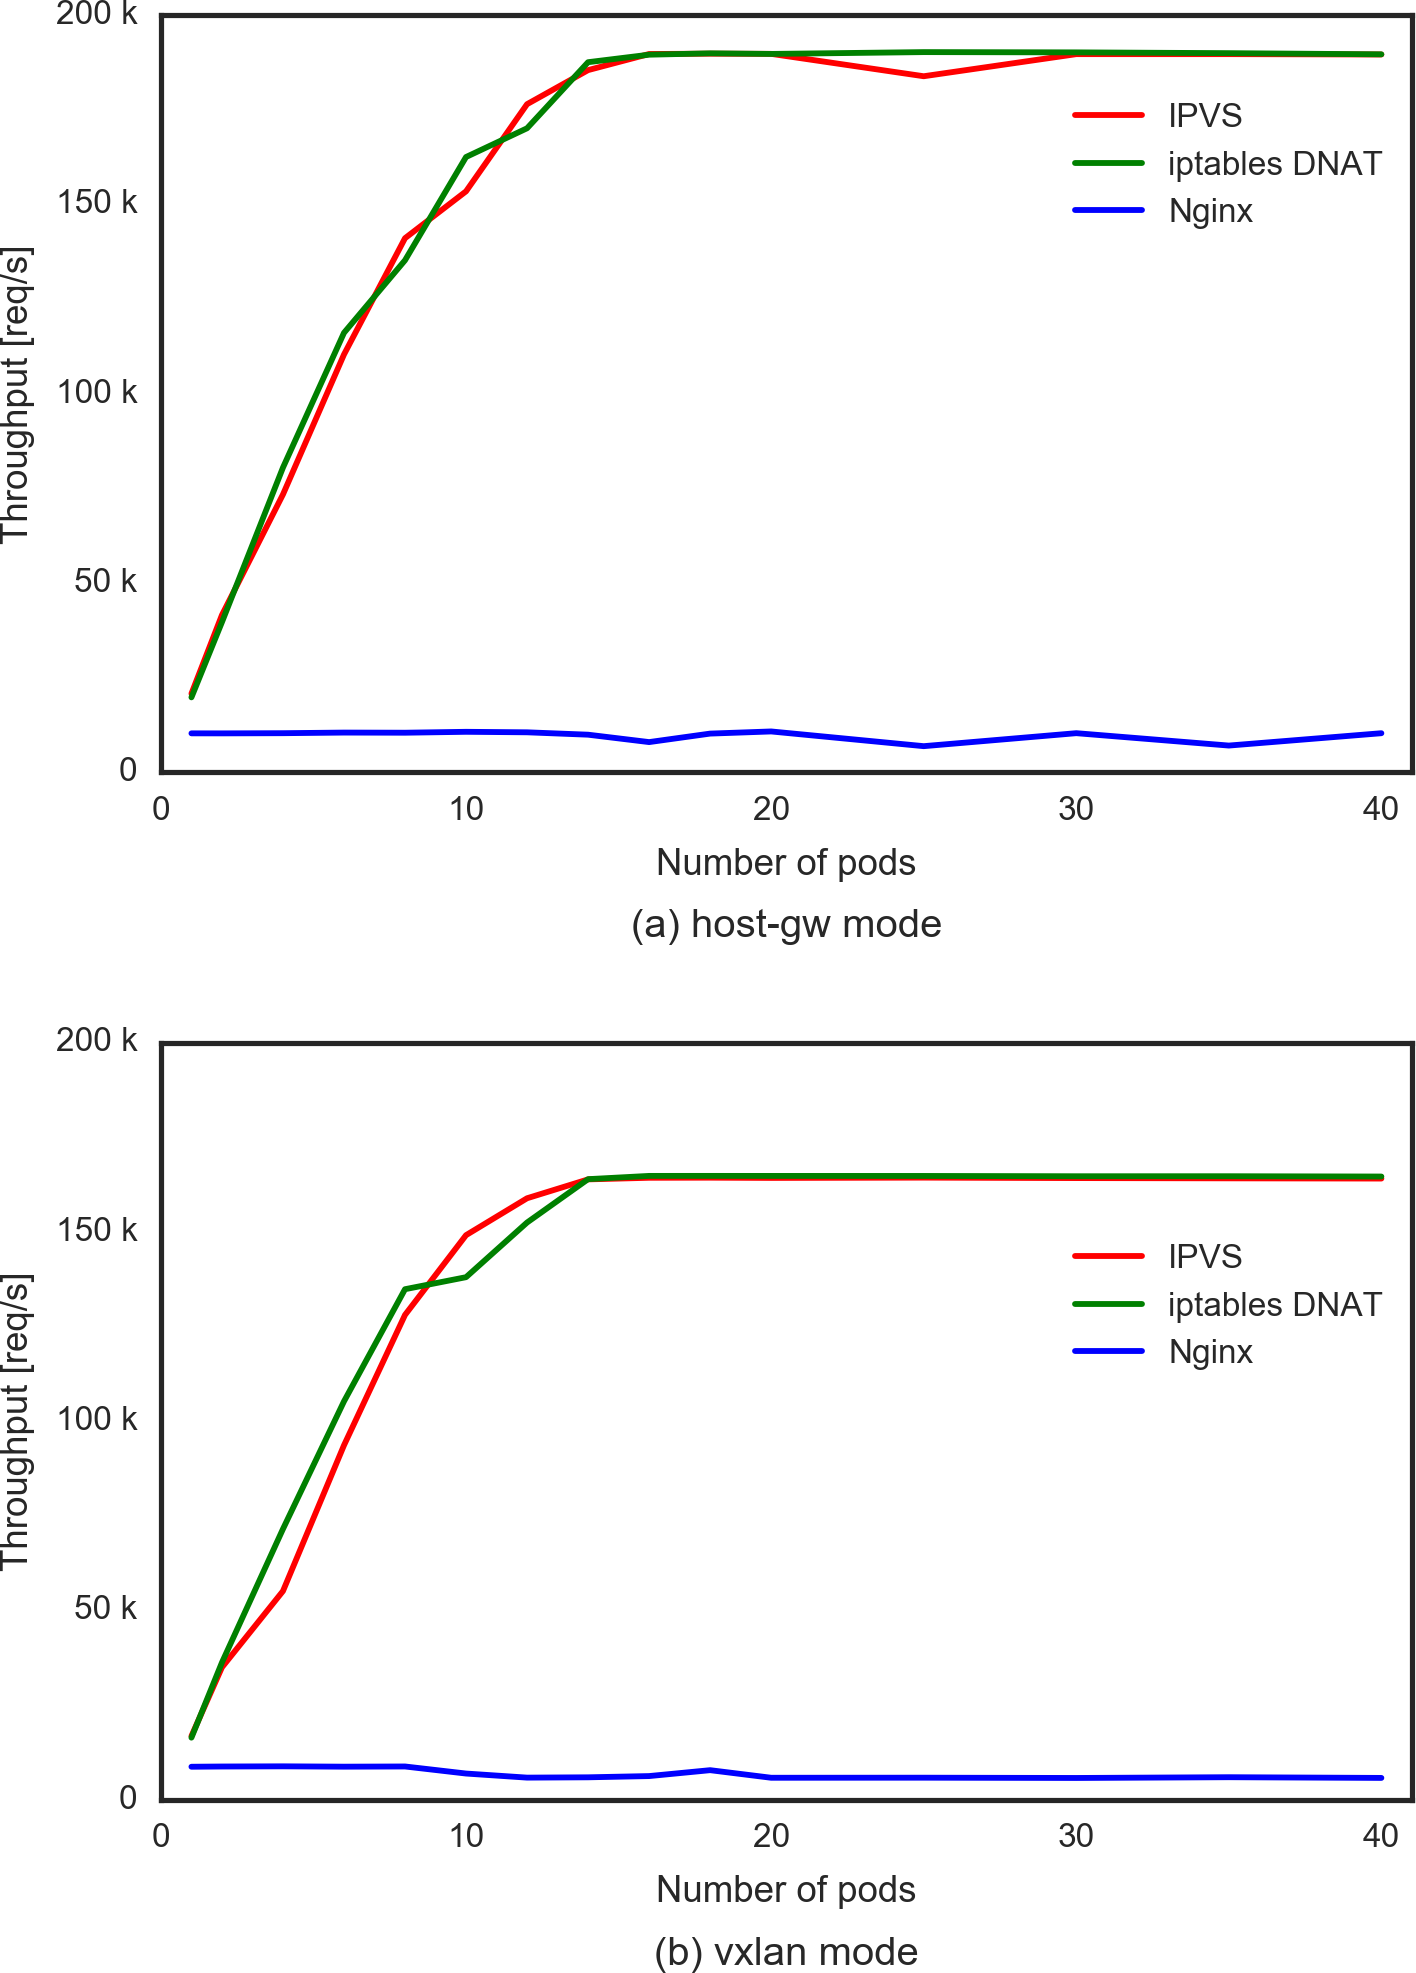
\includegraphics[width=\columnwidth]{Figs/ipvs-iptables-nginx_2figs}
\caption{IPVS and iptables comparison}
\label{fig:IPVS-iptables-nginx_2figs}
\end{figure}

\begin{figure}
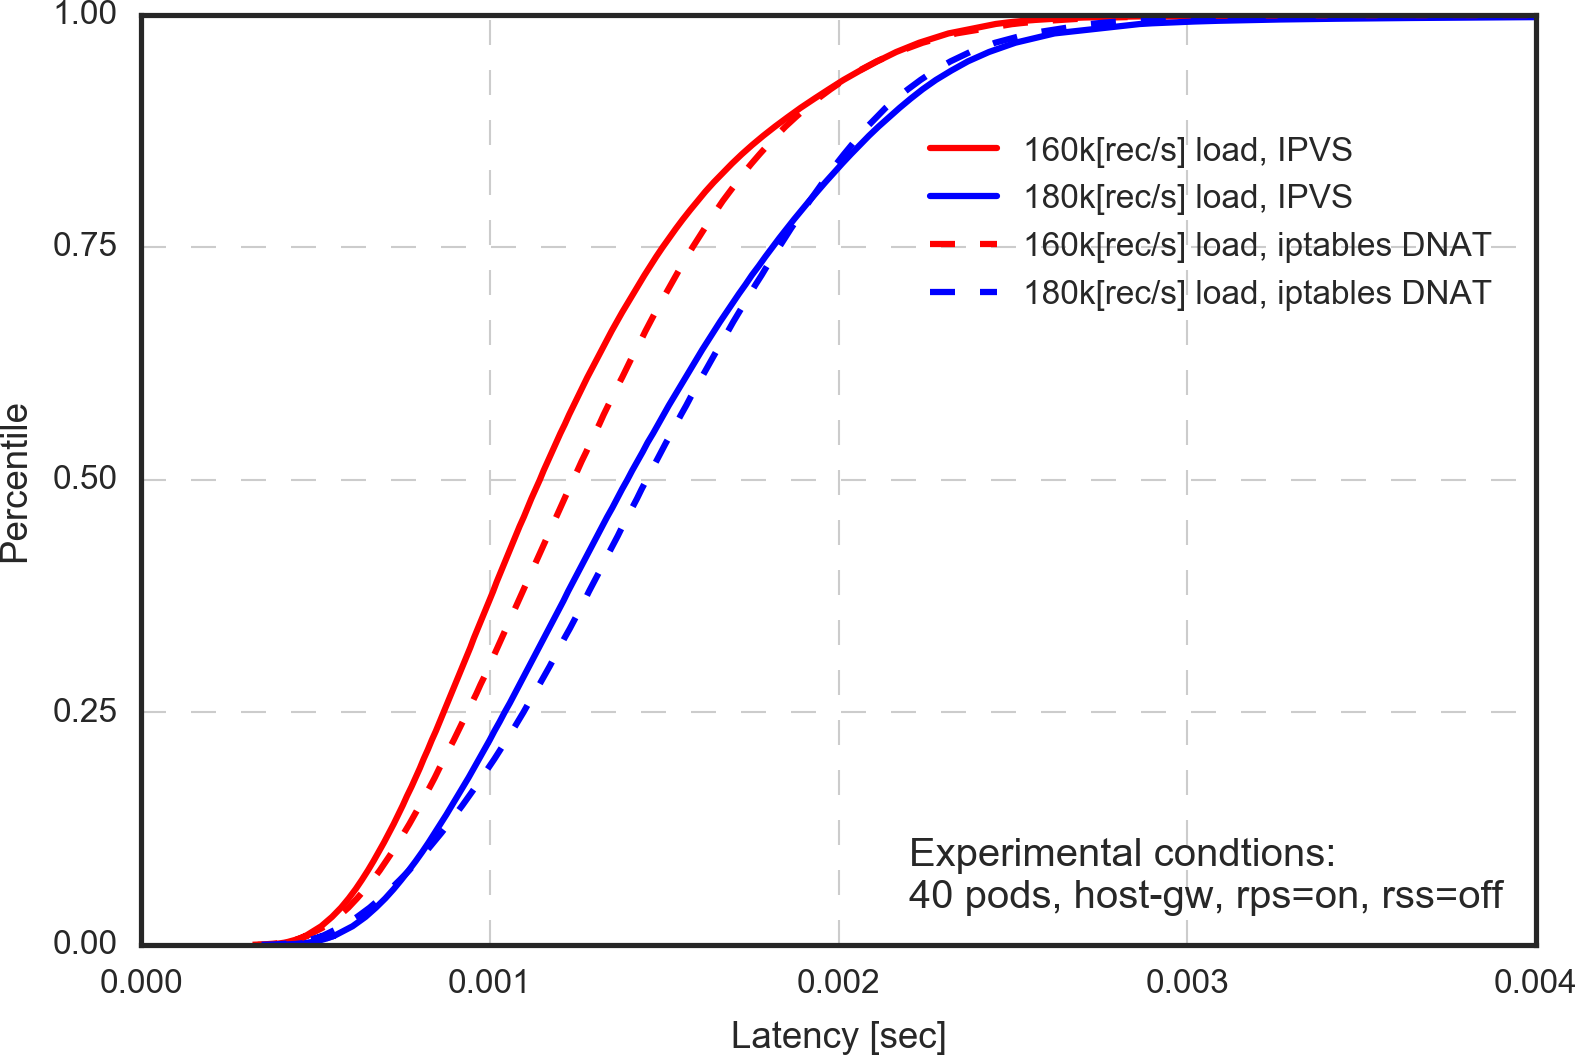
\includegraphics[width=\columnwidth]{Figs/latency_cdf_rps_40pods}
\caption{Latency cumulative distribution function}
\label{fig:latency_cdf_rps_40pods}
\end{figure}

\section{Conclusions}\label{Conclusions}

In this paper, we proposed a portable software load balancer that has the following features, 1) runnable as a Linux container, 2) redundancy with ECMP technique,  for the container cluster systems.

Our load balancer aims at facilitating migration of container clusters for web services.
We implemented a containerized software load balancer that is run by Kubernetes as a part of container cluster,
using Linux kernel's IPVS.

To discuss the feasibility of the proposed load balancer, we built
a Kubernetes cluster system and conducted performance measurements.
Our experimental results indicate that the IPVS based load balancer in container improves the portability of
the container cluster while it shows the similar performance levels as the existing iptables DNAT based load balancer.

We also started to the implementation of a novel software load balancer using recently introduced Linux kernel's XDP infrastructure.
While it is in a preliminary stage of the development, essential functions and design issues have been already clarified.
They will be presented at the time of the presentation.

\section{Future work}\label{Future work}

We leave the following for the future work:
1) Performance measurement of XDP load balancer
2) Implementation of consistent hashing balancing algorithm
3) Containerization of XDP load balancer
These works are ongoing and will be presented when they are available.

